\documentclass{scrartcl}

%%%%%%%%%%%%%%%%%%%%%%%%%%%%%%%%%%%%%%%
%% Makros & anderer Low-Level bastel %%
%%%%%%%%%%%%%%%%%%%%%%%%%%%%%%%%%%%%%%%
\makeatletter
%% Makros für Titel, Autor und Datum 
%% Dank diesem Makro stehen Titel, Autor und Datum überall im Dokument zur verfügung
%% Date hat zudem den Default-Wert \today
\def\@Title{}
\def\@Author{}
\def\@Date{\today}
\newcommand{\Title}{\@Title}
\newcommand{\Author}{\@Author}
\newcommand{\Date}{\@Date}
\AtBeginDocument{%
  \let\@Title\@title
  \let\@Author\@author
  \let\@Date\@date
}

%% Makros für den Arraystretch (bei uns meist in Tabellen genutzt, welche Formeln enthalten)
% Default Value
\def\@ArrayStretchDefault{1} % Entspricht der Voreinstellung von Latex

% Setzt einen neuen Wert für den arraystretch
\newcommand{\setArrayStretch}[1]{\renewcommand{\arraystretch}{#1}}

% Setzt den arraystretch zurück auf den default wert
\newcommand{\resetArrayStretch}{\renewcommand{\arraystretch}{\@ArrayStretchDefault}}

% Makro zum setzten des Default arraystretch. Sollte nur in der Präambel verwendet werden.
\newcommand{\setDefaultArrayStretch}[1]{\def\@ArrayStretchDefault{#1}\renewcommand{\arraystretch}{#1}}
\makeatother


%%%%%%%%%%%%%%
%% Packages %%
%%%%%%%%%%%%%%
\usepackage[utf8]{inputenc} % UTF-8 unterstützung
\usepackage[ngerman]{babel} % Silbentrennung
\usepackage[automark]{scrpage2} % Header und Footer
\usepackage{keystroke} % Keystoke Fonts
\usepackage{listings}
\usepackage{tabularx}


%%%%%%%%%%%%%%%%%%%%%%%%%%%%%%%%%%%
%% Layout der Kopf und Fusszeile %%
%%%%%%%%%%%%%%%%%%%%%%%%%%%%%%%%%%%
\deftripstyle{bericht}[0pt][0.5pt]
	{\Title}	% Kopfzeile innen
	{\headmark}	% Kopfzeile mitte
	{\pagemark}	% Kopfzeile aussen
	{\Author}	% Fusszeile innen
	{}			% Fusszeile mitte
	{\Date}	% Fusszeile aussen
\pagestyle{bericht}

\ifx \GUARDhsrColors \undefined
\def\GUARDhsrColors{}

\usepackage[table]{xcolor}

\definecolor{HSRWhite}{cmyk}{0,0,0,0}

\definecolor{HSRBlue}{cmyk}{1,0.4,0,0.2}
\definecolor{HSRBlue80}{cmyk}{0.8,0.32,0,0.16}
\definecolor{HSRBlue60}{cmyk}{0.6,0.24,0,0.12}
\definecolor{HSRBlue40}{cmyk}{0.4,0.16,0,0.08}
\definecolor{HSRBlue20}{cmyk}{0.2,0.08,0,0.04}

\definecolor{HSRLightGray}{cmyk}{0,0,0,0.30}
\definecolor{HSRLightGray80}{cmyk}{0,0,0,0.24}
\definecolor{HSRLightGray60}{cmyk}{0,0,0,0.18}
\definecolor{HSRLightGray40}{cmyk}{0,0,0,0.12}
\definecolor{HSRLightGray20}{cmyk}{0,0,0,0.06}

\definecolor{HSRSchwarz}{cmyk}{0,0,0,1}
\definecolor{HSRSchwarz80}{cmyk}{0,0,0,0.8}
\definecolor{HSRSchwarz60}{cmyk}{0,0,0,0.6}
\definecolor{HSRSchwarz40}{cmyk}{0,0,0,0.4}
\definecolor{HSRSchwarz20}{cmyk}{0,0,0,0.2}

\definecolor{HSRHematite}{cmyk}{0.6,1,0.4,0.2}
\definecolor{HSRHematite80}{cmyk}{0.48,0.80,0.32,0.16}
\definecolor{HSRHematite60}{cmyk}{0.36,0.60,0.24,0.12}
\definecolor{HSRHematite40}{cmyk}{0.24,0.40,0.16,0.08}
\definecolor{HSRHematite20}{cmyk}{0.12,0.20,0.08,0.04}

\definecolor{HSRLakeGreen}{cmyk}{0.70,0.30,0.45,0.05}
\definecolor{HSRLakeGreen80}{cmyk}{0.56,0.24,0.36,0.03}
\definecolor{HSRLakeGreen60}{cmyk}{0.42,0.18,0.27,0.02}
\definecolor{HSRLakeGreen40}{cmyk}{0.28,0.06,0.13,0.06}
\definecolor{HSRLakeGreen20}{cmyk}{0.14,0.06,0.09,0.01}

\definecolor{HSRReed}{cmyk}{0.10,0.25,0.45,0.60}
\definecolor{HSRReed80}{cmyk}{0.08,0.20,0.36,0.48}
\definecolor{HSRReed60}{cmyk}{0.06,0.15,0.27,0.36}
\definecolor{HSRReed40}{cmyk}{0.04,0.10,0.18,0.24}
\definecolor{HSRReed20}{cmyk}{0.02,0.05,0.09,0.12}

\definecolor{HSRPetrol}{cmyk}{1,0.18,0,0.45}
\definecolor{HSRPetrol80}{cmyk}{0.64,0.08,0.12,0.32}
\definecolor{HSRPetrol60}{cmyk}{0.48,0.06,0.09,0.24}
\definecolor{HSRPetrol40}{cmyk}{0.32,0.04,0.06,0.16}
\definecolor{HSRPetrol20}{cmyk}{0.16,0.02,0.03,0.08}

\definecolor{HSRBasswood}{cmyk}{0.25,0.05,0.70,0.15}
\definecolor{HSRBasswood80}{cmyk}{0.20,0.04,0.56,0.12}
\definecolor{HSRBasswood60}{cmyk}{0.15,0.03,0.42,0.09}
\definecolor{HSRBasswood40}{cmyk}{0.10,0.02,0.28,0.06}
\definecolor{HSRBasswood20}{cmyk}{0.05,0.01,0.14,0.03}


\fi
\ifx\GUARDmathe\undefined
\def\GUARDmathe{}

\usepackage{amssymb}
% Das mathtools package ist eine Erweiterung zum amsmath package.
% Das amsmath package wird dabei automatisch geladen
\usepackage{mathtools}

\fi

% Seitenränder für Formelsammlungen
\usepackage[left=1cm,right=1cm,top=1cm,bottom=1cm,includeheadfoot]{geometry}


% Makros für Verweise auf ein Buch oder Skript
\newcommand{\buch}[1]{$_{\textcolor{HSRLakeGreen}{\mbox{\small{ #1}}}}$}
\newcommand{\skript}[1]{$_{\textcolor{HSRReed}{\mbox{\small{ #1}}}}$}

\setlength{\parindent}{0pt}
\ifx \GUARDhyperref \undefined
\def\GUARDhyperref{}

\ifx \GUARDhsrColors \undefined
\def\GUARDhsrColors{}

\usepackage[table]{xcolor}

\definecolor{HSRWhite}{cmyk}{0,0,0,0}

\definecolor{HSRBlue}{cmyk}{1,0.4,0,0.2}
\definecolor{HSRBlue80}{cmyk}{0.8,0.32,0,0.16}
\definecolor{HSRBlue60}{cmyk}{0.6,0.24,0,0.12}
\definecolor{HSRBlue40}{cmyk}{0.4,0.16,0,0.08}
\definecolor{HSRBlue20}{cmyk}{0.2,0.08,0,0.04}

\definecolor{HSRLightGray}{cmyk}{0,0,0,0.30}
\definecolor{HSRLightGray80}{cmyk}{0,0,0,0.24}
\definecolor{HSRLightGray60}{cmyk}{0,0,0,0.18}
\definecolor{HSRLightGray40}{cmyk}{0,0,0,0.12}
\definecolor{HSRLightGray20}{cmyk}{0,0,0,0.06}

\definecolor{HSRSchwarz}{cmyk}{0,0,0,1}
\definecolor{HSRSchwarz80}{cmyk}{0,0,0,0.8}
\definecolor{HSRSchwarz60}{cmyk}{0,0,0,0.6}
\definecolor{HSRSchwarz40}{cmyk}{0,0,0,0.4}
\definecolor{HSRSchwarz20}{cmyk}{0,0,0,0.2}

\definecolor{HSRHematite}{cmyk}{0.6,1,0.4,0.2}
\definecolor{HSRHematite80}{cmyk}{0.48,0.80,0.32,0.16}
\definecolor{HSRHematite60}{cmyk}{0.36,0.60,0.24,0.12}
\definecolor{HSRHematite40}{cmyk}{0.24,0.40,0.16,0.08}
\definecolor{HSRHematite20}{cmyk}{0.12,0.20,0.08,0.04}

\definecolor{HSRLakeGreen}{cmyk}{0.70,0.30,0.45,0.05}
\definecolor{HSRLakeGreen80}{cmyk}{0.56,0.24,0.36,0.03}
\definecolor{HSRLakeGreen60}{cmyk}{0.42,0.18,0.27,0.02}
\definecolor{HSRLakeGreen40}{cmyk}{0.28,0.06,0.13,0.06}
\definecolor{HSRLakeGreen20}{cmyk}{0.14,0.06,0.09,0.01}

\definecolor{HSRReed}{cmyk}{0.10,0.25,0.45,0.60}
\definecolor{HSRReed80}{cmyk}{0.08,0.20,0.36,0.48}
\definecolor{HSRReed60}{cmyk}{0.06,0.15,0.27,0.36}
\definecolor{HSRReed40}{cmyk}{0.04,0.10,0.18,0.24}
\definecolor{HSRReed20}{cmyk}{0.02,0.05,0.09,0.12}

\definecolor{HSRPetrol}{cmyk}{1,0.18,0,0.45}
\definecolor{HSRPetrol80}{cmyk}{0.64,0.08,0.12,0.32}
\definecolor{HSRPetrol60}{cmyk}{0.48,0.06,0.09,0.24}
\definecolor{HSRPetrol40}{cmyk}{0.32,0.04,0.06,0.16}
\definecolor{HSRPetrol20}{cmyk}{0.16,0.02,0.03,0.08}

\definecolor{HSRBasswood}{cmyk}{0.25,0.05,0.70,0.15}
\definecolor{HSRBasswood80}{cmyk}{0.20,0.04,0.56,0.12}
\definecolor{HSRBasswood60}{cmyk}{0.15,0.03,0.42,0.09}
\definecolor{HSRBasswood40}{cmyk}{0.10,0.02,0.28,0.06}
\definecolor{HSRBasswood20}{cmyk}{0.05,0.01,0.14,0.03}


\fi

\usepackage[plainpages=false,pdfpagelabels]{hyperref}
\hypersetup{
  pdfstartview={FitH}, % fits the width of the page to the window
  pdfauthor={\Author},
  pdfcreator={\Author},
  pdfproducer={\Author},
  pdftitle={\Title},
  colorlinks=true,
  linkcolor=HSRBlue,
  citecolor=HSRDeer,
  filecolor=HSRLake,
  urlcolor=HSRHematite
}

\fi
\usepackage{tikz}
\usepackage{circuitikz}
\usepackage{adjustbox} % Doku: http://mirror.switch.ch/ftp/mirror/tex/macros/latex/contrib/adjustbox/adjustbox.pdf
\usepackage{longtable}

\setDefaultArrayStretch{1.8}

\title{MikroelSys1}
\author{Jürg Rast, Gian Claudio Köppel}


\begin{document}

\section{Für Anina}
\subsection{Kleine Kunde der Anglosächsischen Sprache}
\begin{tabular}{lll}
	Inversion & Inwörschn & allgemein für die Umkehr einer Sache \\
	Invasion & Inwäischn & a military action of soldiers entering a foreign land\\
\end{tabular}
\subsection{Nützliche hinweise für die Prüfung}
\begin{itemize}
  \item Luag mal!
  \item Lappi tua d Auga uf!
  \item Nimm no d Tomata vo da Auga.
\end{itemize}
\subsection{Wann leitet was?}
\begin{itemize}
  \item P leitet wenn Eingang gegen 0 ist
  \item N leitet wenn Eingang gegen 1 ist
\end{itemize}


\section{CMOS Technologie\skript{Kap. 3}}
\subsection{Chipherstellung}
\subsubsection{5 Hauptschritte der Herstellung}
\begin{enumerate}[nosep, noitemsep]
  \item Oberflächenbeschichtung
  \item Fotolithografie
  \item Ätzen
  \item Dotieren
  \item Säubern der Wafer
\end{enumerate}


\section{Schaltungselemente in CMOS\skript{Kap. 4}}
\setArrayStretch{1}
\begin{tabular}{ll}
Absolute Genauigkeit: & $\pm 20 \%$ \\
Relative Genauigkeit: & $\pm 1\%$
\end{tabular}
\setArrayStretch{1.8}

\subsection{Kapazitäten}
\setArrayStretch{1}
\begin{tabular}{ll}
	Poly-Poly-Kapazität & $C'' \approx 1fF/\mu m^2$ \\
	MOS-Kapazität & $C'' \approx 10fF/\mu m^2$ \\
	MIM-Kapazität (Metall-Isolator-Metall) &  $C'' \approx 1fF/\mu m^2$
\end{tabular}
\setArrayStretch{1.8}

$C''$:  spezifische Kapazität pro Flächeneinheit. \\
$d$: Plattenabstand (meist durch Herstellung gegeben). \\

\begin{tabularx}{\linewidth}{|l|X|}
	\hline
	Elektrische Feldkonstante	& $\epsilon_0 = 8.85 \cdot 10^{-12} F/m$
	\\ \hline
	Siliziumdioxid & $\epsilon_r = 3.9$
	\\ \hline
	Kapazität/Fläche	& $C'' = \cfrac{\epsilon}{d} = \cfrac{\epsilon_0 \epsilon_r}{d}$
	\\ \hline
	Kapazität & $C = C'' \cdot A$
	\\ \hline
\end{tabularx}

\subsection{Widerstände}
Unerwünscht, da hoher Platzbedarf und Wärme.

\[
	R = R_\diamond \frac{L}{W}
\]
{
\centering
\begin{tabularx}{0.8\linewidth}{|l|l|X|l|l|}
	\hline
	\multicolumn{5}{|c|}{\textbf{Typische Werte für Widerstände}}
	\\ \hline
	Poly-Widerstand & $R \approx 10 \Omega/\diamond$ & & HR-Poly-Widerstand & $R \approx 1k\Omega/\diamond$
	\\ \hline
	P-Diffusions-Widerstand & $R \approx 100\Omega/\diamond$ & & N-Diffusions-Widerstand & $R \approx 100\Omega/\diamond$
	\\ \hline
	N-Well-Widerstand & $R \approx 1k\Omega/\diamond$ & & &
	\\ \hline
\end{tabularx} \\
}

\section{MOS-Transistoren\skript{Kap. 5}}

\subsection{Allgemeine Begriffe und Formeln}

%\begin{tabular}{|l|l|l|}
%	\hline
%	$V_T$			& Schwellenspannung		& Threshold Voltage
%	\\ \hline
%	$V_{DS,sat}$	& Sättigungsspannung	&
%	\\ \hline
%	$a_A$			& Early-Faktor			&
%	\\ \hline
%	$\lambda$		& Kanallängen Modulationsfaktor & $\lambda = \frac{1}{V_A}$, \quad $I_{D,real} = I_{D,ideal}(1 + \lambda V_{DS})$
%	\\ \hline
%	$V_A$			& Early-Spannung		& $V_A \approx a_A \cdot L$ \quad $V_{A}$ ist immer positiv
%	\\ \hline
%	$\Phi_t$		& Temperaturspannung	& $\Phi_t = V_{temp} = \frac{kT}{e} \quad k = 1.38 \cdot 10^{23} J/K \quad e=1.6 \cdot 10^{-19} C$
%	\\ \hline
%	$r_{DS}$		& Ausgangswiderstand	& $r_{DS} = \frac{1}{g_0} \approx \frac{\Delta V_{DS}}{\Delta I_D} \quad 
%											  \text{oder} \quad r_{DS} = \frac{V_A + V_{DS}}{I_{D,real}} \approx \frac{V_A}{I_D} $ 
%	\\				&						&$V_{A}, V_{DS}, I_{D,real}$ immer im Betrag rechnen
%	\\ \hline
%	
%\end{tabular}

\subsection{Inversion}

\begin{tabular}{|l|l|l|}
	\hline
	\textbf{Arbeitsbereich}	& \textbf{Bedingung}					& \textbf{Sättigungspannung}
	\\ \hline
	weak inversion			& $0 < V_{GS} < V_T - 60mV$				& $V_{DS,sat} \approx 5\Phi_t \approx 130mV \quad \text{(bei } T = 300K \text{)}$ 
	\\ 						&										& $V_{GS} = V_{M} + h_{M} \cdot \Phi_t \cdot 																\ln{\frac{I_{D}}{\frac{W}{L} \cdot I_{M}}}$ 
	\\ \hline
	moderate inversion		& $V_T - 60mV < V_{GS} < V_T + 160mV$	&
	\\ \hline
	strong inversion		& $V_T + 160mV < V_{GS} $				& $V_{DS,sat} = V_{GS} - V_T = \sqrt{\frac{{2 I_{D}}}{\beta}} = 																	\sqrt{\frac{2 I_{D}}{\frac{W}{L} \cdot \beta_{0}}}$
	\\ \hline
\end{tabular}


\subsection{Betriebsarten}
Achtung: Beim Bipolar Transistor wird der Bereich links der Sättigungsgrenze als Sättigungsbereich bezeichnet, beim MOS-Transistor ist es der Bereich
rechts der Sättigungsgrenze!

\begin{figure}[h]
	\centering
	\begin{subfigure}[b]{6cm}
		\centering
		\adjustbox{scale=0.7}{\begin{circuitikz}[american, european resistors]
	\draw (1.5,0) node[circ, name=G] {} node[right] {G};
	\draw (4,0) node[circ, name=D] {} node[right] {D};
	\draw (4,-2) node[circ, name=S] {} node[right] {S};
	\draw (0,-2) -- (S);
	\draw (G) -- +(-1.5,0);
	\draw (3,0) to[R=$r_{DS0}$] +(0,-2);
	\draw (0,-2) to[V] ++(0,2) ;
	\draw (0,-2) -- + (0,-0.2) node[ground] {};
	\draw (D) -- +(-1,0);
	\draw[->, thick] (-0.9, -0.2) -- +(0,-1.4) node[midway, left] {$V_{GS}$};
\end{circuitikz}}
		\caption{Widerstandsbetrieb}
	\end{subfigure} \qquad\qquad
	\begin{subfigure}[b]{7cm}
		\centering
		\adjustbox{scale=0.7}{\begin{circuitikz}[american, european resistors]
	\draw (1.5,0) node[circ, name=G] {} node[right] {G};
	\draw (5,0) node[circ, name=D] {} node[right] {D};
	\draw (5,-2) node[circ, name=S] {} node[right] {S};
	\draw (0,-2) -- (S);
	\draw (G) -- +(-1.5,0);
	\draw (4,0) to[R=$r_{DS}$] +(0,-2);
	\draw (3,0) to[I,mirror,l=$g_mV_{GS}$] +(0,-2);
	\draw (0,-2) to[V] ++(0,2) ;
	\draw (0,-2) -- + (0,-0.2) node[ground] {};
	\draw (D) -- ++(-1,0) to[short, i_=$I_D$] +(-1,0);
	\draw[->, thick] (-0.9, -0.2) -- +(0,-1.4) node[midway, left] {$V_{GS}$};
\end{circuitikz}}
		\caption{Stromquellenbetrieb}
	\end{subfigure}
	\caption{Ersatzschlatbilder MOS-Transistoren}
\end{figure}

\subsubsection{Ungesättigter Betrieb}
Bei $V_{DS} = 0$ verhält sich der Kanal wie ein Widerstand. Die Kennlinie ist eine Gerade durch den Ursprung. Je steiler diese Gerade ist, desto
kleiner ist der Widerstand $r_{DS}$.

\subsubsection{Gesättigter Betrieb}
Bei $V_{DS} \geq V_{DS,sat}$ verhält sich der Kanal wie eine Stromquelle. Wenn die Geraden horizontal verlaufen ist $r_{DS} = \infty$ und
es handelt sich um einen idealen Transistor. Beim realen Transistor steigen jedoch diese Geraden immer leicht an.
Der Anstieg entspricht dem \textbf{Ausgangsleitwert} $g_0$, respektive dem \textbf{Ausgangswiderstand} $r_{DS}$.
Andere Bezeichnungen: differentieller- , Kleinsignal-, dynamischer Ausgangswiderstand.
\[
	r_{DS} = \frac{1}{g_0} = \frac{dV_{DS}}{dI_{D}} \approx \frac{\Delta V_{DS}}{\Delta I_D}
\]

Der Kanal-Widerstand kann auch mit Hilfe der Early-Spannung berechnet werden:
\[
	r_{DS} = \frac{V_A + V_{DS}}{I_{Dreal}} \quad \stackrel{V_A >> V_{DS}}{\approx} \quad \frac{V_A}{I_D}
\]

\subsection{Transferkennlinie}


\begin{figure}[h]
	\centering
	\begin{subfigure}[b]{0.33\textwidth}
		\centering
\adjustbox{scale=0.8}{\begin{tikzpicture}

\draw [->] (0,0) -- (0,5) node [anchor=south] {$I_D$};
\draw [->] (0,0) -- (8,0) node [anchor=west] {$V_{GS}$};

\draw [color=red, thick] (0,0) -- (1,0);
\draw [color=orange, very thick] (1,0) -- (3,0);
\draw [color=yellow, thick] (3,0) arc (-90:-78:5);
\draw [color=green, very thick] (4.0,0.1) .. controls (5,0.25) and (5.5,1.2) .. (6,2);
\draw [color=blue] (6,2) -- (7,4.5);
\draw (6,2) -- (7,4);

\node [color=blue] at (5,4) {Effektiver Verlauf}; 
\node at (9,3.5) {Exakt linearer Verlauf};


\foreach \x in {1,3,4,6} {
	\draw (\x,0.1) -- (\x,-0.1);
	\draw (\x,-0.7) -- (\x,-1.3);
}

\draw (3.5,0.1) -- (3.5,-0.1);

\draw (0,-0.7) rectangle (7,-1.3);

\node at (1,0) [anchor=north] {$V_K$};
\node at (3,0) [anchor=north] {$V_M$};
\node at (3.5,0) [anchor=north] {$V_T$};
\node at (4,0) [anchor=north] {$V_H$};
\node at (6,0) [anchor=north] {$V_L$};

\node at (0.5,-1) {0};
\node at (2,-1) {1 EXP};
\node at (3.5,-1) {2};
\node at (5,-1) {3 QUAD};
\node at (6.5,-1) {4};

\draw (0,-1.7) rectangle (7,-2.3);
\draw (3.5,-1.7) -- (3.5,-2.3);
\node at (1.75,-2) {Subthreshold};
\node at (3.5+1.75,-2) {Above Threshold};
\end{tikzpicture}}
	\end{subfigure} \qquad\qquad
	\begin{subfigure}[b]{0.58\textwidth}
		{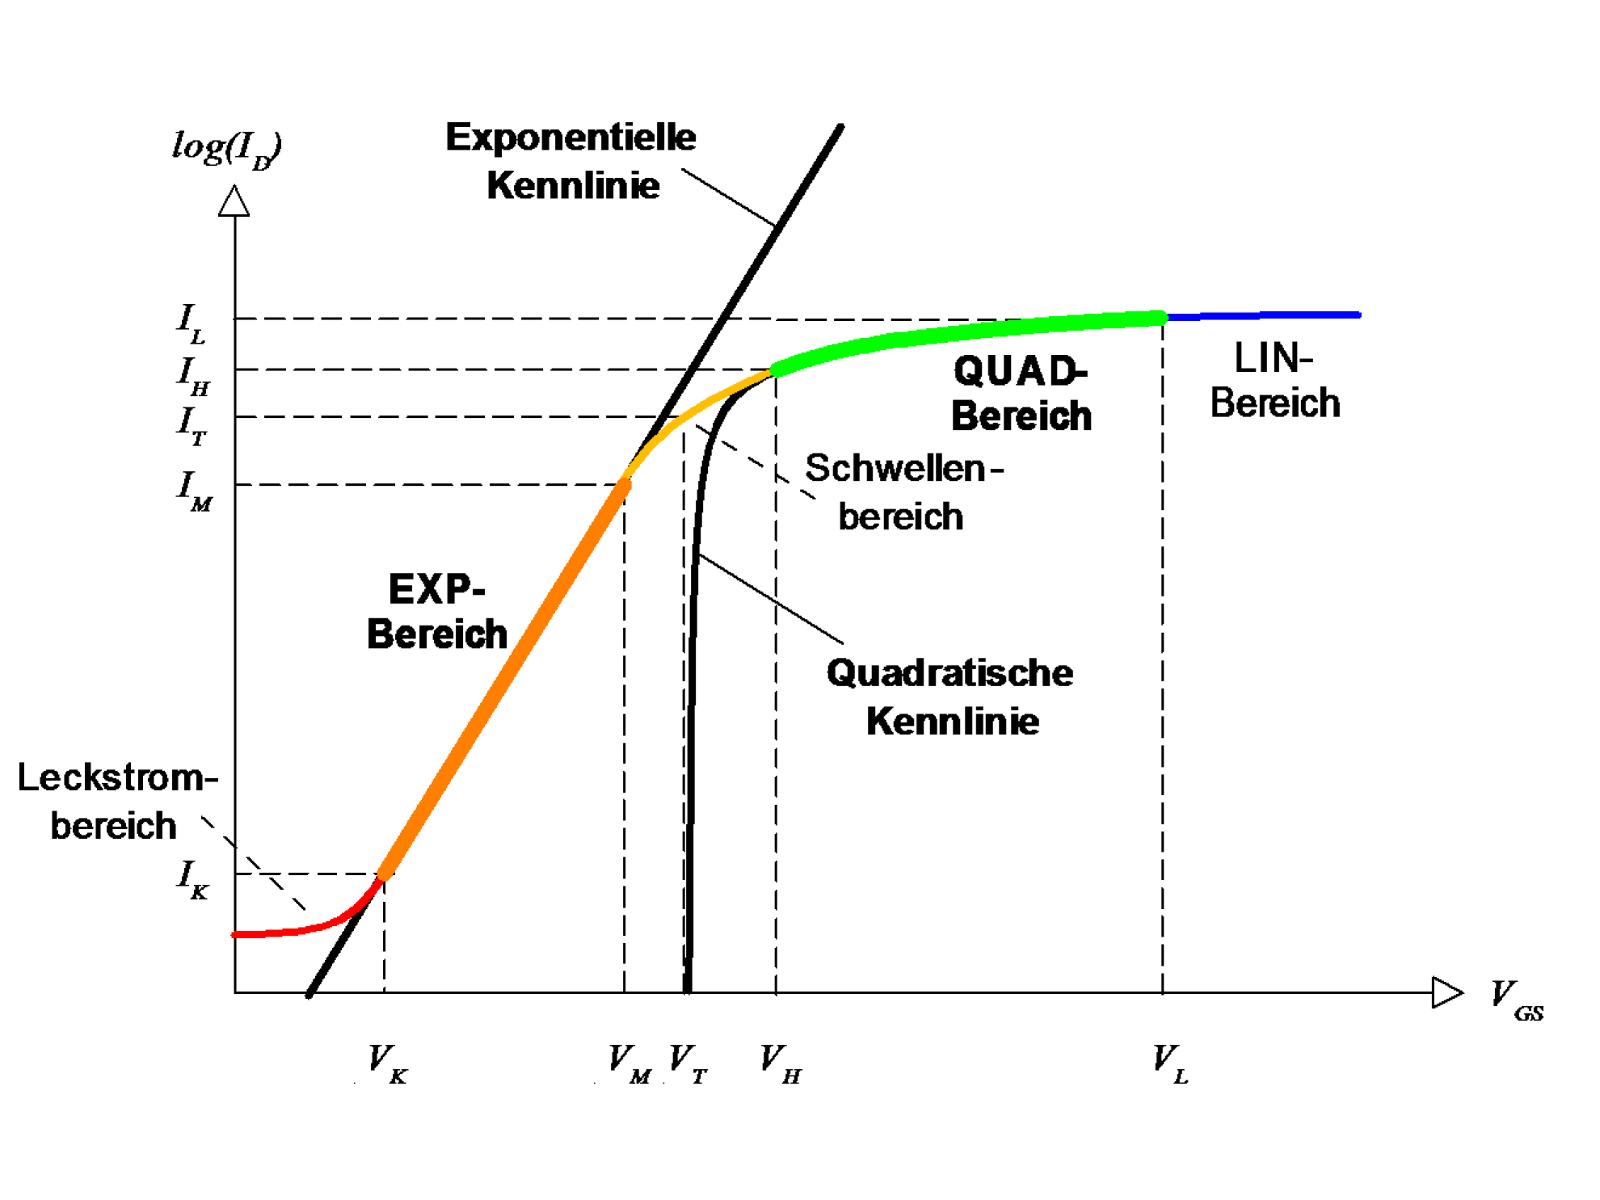
\includegraphics[width=\textwidth]{images/Transferkennlinie.png}}
		\centering

	\end{subfigure}
\end{figure}




\setArrayStretch{1.1}
\begin{tabular}{|lp{3cm}|p{6cm}|p{8cm}|}
	\hline
	& \textbf{Ausgangs\-strom\-bereich} & \textbf{Mathematische Charakterisierung} & \textbf{Zugrundeliegender physikalischer Effekt}
	\\ \hline
	\cellcolor{red!70}
	0 
	& Leckstrombereich (LECK) 
	& $I_D$ erreicht Minimalwert, der nicht weiter unterschritten werden kann
	& Drain-Substratdiode und Source-Substratdiode haben Leckströme im Substrat
	\\ \hline
	\cellcolor{orange!70}
	1
	& Exponentieller Bereich (EXP)
	& $I_D$ steigt exponentiell mit $V_{GS}$
	& Kanal zeigt schwache Inversion (Beim n-Kanal-Transistor: Ursprünglich p-leitender Kanal ist schwach n-leitend)
	\\ \hline
	\cellcolor{yellow!70}
	2
	& Schwellen Bereich (MOD)
	& Keine "`handlichen"' Formel für $I_D$ vorhanden
	& Kanal zeigt moderate Inversion (Kanalzustand liegt zwischen schwacher und starker Inversion)
	\\ \hline
	\cellcolor{green!70}
	3
	& Quadratischer Bereich (QUAD)
	& $I_D$ steigt quadratisch mit $V_{GS}$
	& Kanal zeigt starke Inversion (Beim n-Kanal-Transistor: Ursprünglich p-leitender Kanal wirk stark n-leitend)
	\\ \hline
	\cellcolor{blue!70}
	4
	& Linearer Bereich (LIN)
	& $I_D$ steigt annähernd linear mit $V_{GS}$ (halb QUAD, halb LIN)
	& Geschwindigkeitsänderung der Ladungsträger im Kanal (die Ladungsträger können nicht weiter beschleunigt werden)
	\\ \hline
\end{tabular}
\resetArrayStretch


\subsection{Drainstromgleichungen}
\setArrayStretch{1.5}
\begin{tabular}{|l|l|l|}
	\hline
		\textbf{Ausgangsstrom} 
		& \multicolumn{2}{c|}{\textbf{Ausgangsspannungsbereich} ($V_{DS}$-Bereich)}
	\\
		($I_D-, V_{GS}$-Bereich)
		& Transistor ungesättigt ($|V_{DS}| < |V_{DS,sat}|$)
		& Transistor gesättigt ($|V_{DS}| > |V_{DS,sat}|$)
	\\ \hline
		\multicolumn{3}{|c|}{\textbf{n-Kanal ohne Kanallängenmodulation und ohne unterschiedlicher Transkonduktanz:}}
	\\ \hline
		EXP-Bereich
		& $I_D = I_M e^{\frac{V_{GS}-V_M}{n_M \Phi_t}} (1-e^{\frac{-V_{DS}}{\Phi_t}})$
		& $I_D = I_M e^{\frac{V_{GS}-V_M}{n_M \Phi_t}}$
	\\ \hline
		QUAD-Bereich
		& $I_D = \beta [(V_{GS} - V_T) V_{DS} - \frac{V_{DS}^2}{2}]$
		& $I_D = \frac{\beta}{2}(V_{GS} - V_T)^2$
	\\ \hline
		\multicolumn{3}{|c|}{\textbf{n-Kanal mit Kanallängenmodulation und mit unterschiedlicher Transkonduktanz:}}
	\\ \hline
		EXP-Bereich
		& $I_D = I_M e^{\frac{V_{GS}-V_M}{n_M \Phi_t}} (1-e^{\frac{-V_{DS}}{\Phi_t}}) (1 + \lambda V_{DS})$
		& $I_D = I_M e^{\frac{V_{GS}-V_M}{n_M \Phi_t}} (1 + \lambda V_{DS})$
	\\ \hline
		QUAD-Bereich
		& $I_D = B [(V_{GS} - V_T) V_{DS} - \frac{V_{DS}^2}{2}] (1 + \lambda V_{DS})$
		& $I_D = \frac{\beta}{2}(V_{GS} - V_T)^2 (1 + \lambda V_{DS})$
	\\ \hline
		\multicolumn{3}{|c|}{\textbf{p-Kanal mit Kanallängenmodulation und mit unterschiedlicher Transkonduktanz:}}
	\\ \hline
		EXP-Bereich
		& $I_D = I_M e^{-\frac{V_{GS}-V_M}{n_M \Phi_t}} (1-e^{\frac{-V_{DS}}{\Phi_t}}) (1 - \lambda V_{DS})$
		& $I_D = I_M e^{-\frac{V_{GS}-V_M}{n_M \Phi_t}} (1 - \lambda V_{DS})$
	\\ \hline
		QUAD-Bereich
		& $I_D = -B [(V_{GS} - V_T) V_{DS} - \frac{V_{DS}^2}{2}] (1 - \lambda V_{DS})$
		& $I_D = -\frac{\beta}{2}(V_{GS} - V_T)^2 (1 - \lambda V_{DS})$
	\\ \hline
\end{tabular}
\newline

Die Sättigungsspannung beträgt im \textbf{EXP-Bereich} $5\Phi_t$, im \textbf{QUAD-Bereich} $V_{GS}-V_T$.

Parameter der Gleichungen:

\begin{tabularx}{\linewidth}{|l|l|X|}
	\hline
		$V_{DS,sat}$	& Sättigungsspannung	&
	\\ \hline
		$a_A$			& Early-Faktor			&
	\\ \hline
		$V_T$ & Schwellenspannung &
		Typisch $0.6V$ beim n-Kanal, resp. $-0.6V$ beim p-Kanal. $V_T$ ist stark von der Source-Bulk-Spannung abhängig (Body-Effekt):
		\[ 
			V_T = V_{T0} \pm \Delta V_T \quad \text{mit} \quad \Delta V_T = \gamma(\sqrt{V_{SB} \pm \Phi_0} -\sqrt{\Phi_0})
		\]
		positives Vorzeichen für n-Kanal, negatives für p-Kanal, $\gamma_N \approx 0.6\sqrt{V}$, $\gamma_P \approx 0.5\sqrt{V}$, $\Phi_{0} = 0.6V$ 
	\\ \hline
		$\Phi_t$ & Temperaturspannung &
		\[
			\Phi_t = V_{Temp} = \frac{kT}{e} = 86.2 \frac{\mu V}{K}T
		\]
		somit ist $\Phi_t = 25.9mV$ bei $T=300^\circ K$ bzw. $27^\circ C$
	\\ \hline
		$I_M$ & Drainstrom &
		Drainstrom an der Grenze zwischen schwacher und moderater Inversion.
		\[
			I_M = \frac{W}{L} \cdot I_M'
		\]
		$I_M'$ ist der spezifische Drainstrom an der Grenze
	\\ \hline
		$n_M$ & Unterschwellen-Neigungsfaktor &
		Der Faktor $n_m$ ist von der Source-Bulk-Spannung $V_{SB}$ abhängig:
		\[
			n_M = 1 + \frac{\gamma}{2 \sqrt{V_{SB} + \Phi_0}}
		\]
		Für $V_{SB} = 0$ erhalten wir $n_M=1.39$. Häufig wird ein Wert von $n_M \approx 1.5$ angegeben.
	\\ \hline
		$V_A$			& Early-Spannung		& $V_A \approx a_A \cdot L$ \quad $V_{A}$ ist immer positiv
	\\ \hline
		$\lambda$ & Kanallängen-Modulationsfaktor &
		inverser Wert der Early-Spannung
		\[
			\lambda = \frac{1}{V_A} \approx \frac{1}{a_A L}
		\]
		Der MOS-Transistor wird vielfach mit $\lambda = 0$ idealisiert, was die Handrechnung vereinfacht.
	\\ \hline
		$B, \beta$ & Transkondukdanz &
		Steilheit, Verstärkungsfaktor. Dieser Faktor ist im gesättigten und ungesättigten Betrieb \textbf{grundsätzlich verschieden}.
	\\ \hline
		$g_{m}$	& Transkonduktanz & Steilheit oder Gate-Steilheit. Beschreibt Zusammenhang zwischen $I_{DS}$ und $V_{GS}$. Mass für die Verstärkung.
	\\ \hline
		$g_{mb}$ & Body-Transkonduktanz & Beschreibt Wirkung des Body-Effekts. Nur im gesättigtem Stromquellenbetrieb von Bedeutung. Berechnung siehe Zbinden Formeln.
	\\ \hline
		$g_{0}$ & Ausgangsleitwert &
	\\ \hline
		$r_{DS}$ & Ausgangswiderstand & $r_{DS} = \frac{1}{g_0} \approx \frac{\Delta 	V_{DS}}{\Delta I_D} \quad 
													  \text{oder} \quad r_{DS} = \frac{V_A + V_{DS}}{I_{D,real}} \approx \frac{V_A}{I_D} $ 
	\\				&			&$V_{A}, V_{DS}, I_{D,real}$ immer im Betrag  
	\\ \hline
		$r_{s}$	& innerer Source-Widerstand & $r_{s} = \frac{1}{g_{m}}$
	\\ \hline
\end{tabularx}


\subsection{Richtgrössen der Gleichungsparameter}
\begin{tabular}{|l|l|l|l|l|l|}
	\hline
	\multirow{2}{*}{Parameter-Name}			& \multirow{2}{*}{Parameter-Symbol}	& \multicolumn{2}{c|}{C175 ($2\mu m$ Technologie)}	& \multicolumn{2}{c|}{C35 ($35\mu m$ Technologie)}
	\\ \cline{3-6}
											&					& n-Kanal				& p-Kanal									& n-Kanal					& p-Kanal
	\\ \hline 			
	Schwellenspannung (bei $V_{BS} = 0$)	& $V_{T0}$			& $0.65V$				& $-0.8V$									& $0.46V$					& $-0.68V$
	\\ \hline
	Spezifische Transkonduktanz				& $\beta_0$			& $80\frac{\mu A}{V^2}$	& $30 \frac{\mu A}{V^2}$					& $170 \frac{\mu A}{V^2}$	& $58 \frac{\mu A}{V^2}$
	\\ \hline
	Early Faktor							& $a_A$				& $17 \frac{V}{\mu m}$	& $16 \frac{V}{\mu m}$						&							&
	\\ \hline
	Unterschwellen Neigungsfaktor			& $n_M$				& 1.5					& 1.5										& 1.3						& 1.3
	\\ \hline		
\end{tabular}




\section{MOS-Diode\skript{Kap. 7}}
Für Kennlinien der MOS-Dioden siehe Abbildung \ref{fig:diodenKennlinien}.
\begin{figure}[h]
	\centering
	\begin{subfigure}[b]{5cm}
		\centering
		\adjustbox{scale=0.7}{\begin{circuitikz}[european voltages]
	\draw (0,0) to[full diode, i=$I_D$] (0,-2);
	\draw[->, thick] (-0.7,-0.2) -- (-0.7,-1.8) node[midway, left] {$V_D$};
\end{circuitikz}}
		\caption{Ideale Diode ($V_F = V_{F0}$)}
	\end{subfigure}
	\begin{subfigure}[b]{4cm}
		\centering
		\adjustbox{scale=0.7}{\begin{circuitikz}[european voltages]
	\draw (0,0) to[full diode, i=$I_D$] (0,-2);
	\draw[->, thick] (-0.7,-0.2) -- (-0.7,-1.8) node[midway, left] {$V_D$};
\end{circuitikz}}
		\caption{Reale Diode}
	\end{subfigure} \quad
	\begin{subfigure}[b]{4cm}
		\centering
		\adjustbox{scale=0.7}{\begin{circuitikz}[european voltages]
	\ctikzset{tripoles/mos style/arrows}
	\draw (0,-1) to[Tnmos, n=n1] (0,0);
	\draw (n1.source) to[short, i=$I_D$] (0,-2);
	\draw (n1.gate) |- (n1.drain) -- +(0,0.5);
	\draw[->, thick] (-1.2,0.5) -- (-1.2,-1.5) node[midway, left] {$V_{GS}$};
\end{circuitikz}}
		\caption{n-Kanal}
	\end{subfigure}
	\begin{subfigure}[b]{4cm}
		\centering
		\adjustbox{scale=0.7}{\begin{circuitikz}[european voltages]
	\ctikzset{tripoles/mos style/arrows}
	\draw (0,-1) to[Tpmos, n=n1] (0,0);
	\draw (n1.source) to[short, i<=$I_D$] +(0,0.4);
	\draw (n1.gate) |- (n1.drain) -- +(0,-0.5);
	\draw[->, thick] (0.5,0) -- +(0,-1.5) node[midway, right] {$V_{GS}$};
\end{circuitikz}}
		\caption{p-Kanal}
	\end{subfigure}
	\hspace{1.5cm}
	
	\begin{subfigure}[b]{4cm}
		\adjustbox{scale=0.7}{\begin{tikzpicture}
	\draw[->] (0,0) -- (0,3.5) node[left] {$I_D$};
	\draw[->] (0,0) -- (3.5,0) node[below] {$V_D$};
	\draw (0, 0.04) -- ++(2,0) -- +(0,3);
\end{tikzpicture}}
	\end{subfigure} \quad
	\begin{subfigure}[b]{4cm}
		\centering
		\adjustbox{scale=0.7}{\begin{tikzpicture}
	\draw[->] (0,0) -- (0,3.5) node[left] {$I_D$};
	\draw[->] (0,0) -- (3.5,0) node[below] {$V_D$};
	\draw (0, 0.04) -- ++(1.2,0);
	\draw (1.2,0.04) .. controls (1.5,0.04) and (1.7,2.8) .. (1.7,2.8);
	\draw (2,3.3) node {$I_D = I_S (e^{\frac{V_D}{\Phi_t}}  -1)$};
\end{tikzpicture}}
	\end{subfigure} \qquad
	\begin{subfigure}[b]{8cm}
		\centering
		\adjustbox{scale=0.7}{\begin{tikzpicture}
	\draw[->] (0,0) -- (0,3.5) node[left] {$I_D$};
	\draw[->] (0,0) -- (3.5,0) node[right] {$V_D$};
	\draw (0, 0.04) -- ++(1.2,0);
	\draw (1.2,0.04) .. controls (2.3,0.04) and (3.5,2.5) .. (3.5,2.5);
	\draw (2,3) node {$I_D = \frac{\beta}{2}(V_{GS} -V_T)^2$};
	\draw (1.2,0.1) -- +(0,-0.2) node[below] {$V_T$};
	\draw (0,0.63) -- ++(2.242,0) --  +(0,-0.63);
	\draw (0,2.5) -- (3,0);
	\draw (-0.1, 2.5) -- +(0.2,0);
	\draw (-0.1, 2.5) node[left] {$\frac{V^+}{R_D}$};
	\draw (3, 0.1) -- +(0, -0.2) node[below] {$V^+$};
\end{tikzpicture}}
	\end{subfigure}			
	\caption{Gegenüberstellung Dioden-Kennlinien}
	\label{fig:diodenKennlinien}
\end{figure}

\begin{figure}[h]
	\centering
	\begin{subfigure}[b]{5cm}
		\centering
		\adjustbox{scale=0.8}{\begin{circuitikz}[american, european resistors]
	\draw (0,0) node[circ, name=G] {} node[left] {G};
	\draw (4,0) node[circ, name=D] {} node[right] {D};
	\draw (4,-2) node[circ, name=S] {} node[right] {S};
	\draw (0,-2) -- (S);
	\draw (G) -- +(3,0);
	\draw (3,0) to[R=$\frac{1}{g_0}$] +(0,-2);
	\draw (2,0) to[I_=$g_m v_{GS}$] +(0,-2);
	\draw (D) to[short, i_=$i_D$] +(-1,0);
	\draw[->, thick] (0, -0.2) -- +(0,-1.6) node[midway, left] {$v_{GS}$};
\end{circuitikz}}
	\end{subfigure} \qquad\qquad
	\begin{subfigure}[b]{3cm}
		\centering
		\adjustbox{scale=0.8}{\begin{circuitikz}[american, european resistors]
	\draw (4,0) node[circ, name=D] {} node[right] {D};
	\draw (4,-2) node[circ, name=S] {} node[right] {S};
	\draw (1.5,-2) -- (S);
	\draw (3,0) to[R=$\frac{1}{g_0}$] +(0,-2);
	\draw (3,0) -- (1.5,0) to[R=$\frac{1}{g_m}$] +(0,-2);
	\draw (D) to[short, i_=$i_D$] +(-1,0);
\end{circuitikz}}
	\end{subfigure} \qquad\qquad
	\begin{subfigure}[b]{2cm}
		\centering
		\adjustbox{scale=0.8}{\begin{circuitikz}[american, european resistors]
	\draw (4,0) node[circ, name=D] {} node[right] {D};
	\draw (4,-2) node[circ, name=S] {} node[right] {S};
	\draw (3,-2) -- (S);
	\draw (3,0) to[R=$\frac{1}{g_m}$] +(0,-2);
	\draw (D) to[short, i_=$i_D$] +(-1,0);
\end{circuitikz}}
	\end{subfigure}
	\caption{Ersatzschaltungen der MOS-Diode}
\end{figure}

\begin{tabular}{|l|l|}
	\hline
	Arbeitspunktstrom einer MOS-Diode mit Wiederstandslast $R_D$
	& $I_D = \frac{\beta}{2} (V_{GS} -V_T)^2 = \frac{V^+ - V_{GS}}{R_D} $
	\\ \hline
	Drain-Source Spannung einer MOS-Diode bei gegebenem Strom
	& $ V_{GS} = V_T + \sqrt{\frac{2I_D}{\beta(1+\lambda V_{DS})}} \approx V_T + \sqrt{\frac{2I_D}{\beta}} $
	\\ \hline
	Innenwiderstand der MOS-Diode
	& $ r_{MD} = \frac{v_{GS}}{i_D} = \frac{1}{g_m + g_0} \approx \frac{1}{g_m} $
	\\ \hline	
\end{tabular}



\section{MOS-Transistor als Stromquelle\skript{Kap. 8}}

\subsection{Strom einer MOS Stromquelle}
$I_D=\frac{\beta}{2}\left(V_{GS}-V_T\right)^2\left(1+\lambda V_{DS}\right)
\approx \frac{\beta}{2}\left(V_{GS}-V_T\right)^2 $
\subsection{Sättigungsspannung}
\textbf{Bei starker Inversion}
$V_{DS,sat}=V_{GS}-V_t=\sqrt{\frac{2I_d}{\beta}}$\\
\textbf{Bei schwacher Inversion} $V_{DS,sat}\approx 5 \Phi_t \approx 130mV$

\begin{sidewaystable}
\begin{tabular}{|l|p{2.5cm}|p{8.5cm}|p{6.5cm}|}
\hline
Schaltung & Konfiguration & Ausganswiderstand $r_0$ & Minimale Ausgangsspannung $V_{0,min}$ 
\\ \hline
\adjustbox{valign=t, padding=1ex}{\begin{circuitikz}[scale=0.5, transform shape, european]
\ctikzset{tripoles/mos style/arrows}

\draw (1.5,3) node[nmos] (nmos) {}
	(nmos.G) to (0,3) to [V_=VG] (0,0) node[ground] {}
	(nmos.S) to [R=RS] (1.5,0) node[ground] {}
	(nmos.D) to [R=RL,i<_=ID] (1.5,5.5) node[ocirc] {}
;
\draw [->] (2.5,3.5) -- (2.5,0);
\draw node at (2.5,1.75) [anchor=west] {Vo};
\draw node at (1.5,5.5) [anchor=south] {VDD=V+};
\end{circuitikz}} &
Einfache Quelle mit 1 Transistor &
$r_{out}=r_{iD}=r_{DS}=\frac{1}{g_0}=\frac{V_A+V_{DS}}{I_D}\approx\frac{V_A}{I_D}$ &
$V_0 > V_{0,min} = V_{DS,sat}$ 
\\ \hline
 & Stromquelle mit Source-Widerstand &
$r_{iD}=r_{DS}\left(1+\frac{R_S}{r_S}+\frac{R_S}{r_{DS}}\right)=\frac{1}{g_0}\left(1+g_mR_S\right)+R_S$
& $V_0 > V_{0,min} = R_SI_D+V_{DS,sat}$
\\ \hline
\adjustbox{valign=t, padding=1ex}{\begin{circuitikz}[scale=0.5, transform shape, european]
\ctikzset{tripoles/mos style/arrows}

\draw (3,2) node[nmos] (M1) {}
	(3,4) node [nmos] (M2) {}
	(M1.D) -- (M2.S)
	(M2.D) to [R=RL] (3,6.5) node [ocirc] {}
	(M1.S) to [R=RS] (3,0) node [ground] {}
	(M2.G) to (0,4) to [V=VG2] (0,0) node [ground] {}
	(M1.G) to (1.4,2) to [V=VG1] (1.4,0) node [ground] {}
;
\draw (3.2,4.7) -- (5.5,4.7);
\draw (3.2,2.7) -- (4.5,2.7);
\draw node at (4,5.5) {ro2};
\draw [->] (4,5.3) -- (4,4.7);
\draw node at (4,3.5) {ro2};
\draw [->] (4,3.3) -- (4,2.7);
\draw [->] (5.2,4.5) -- (5.2,0);
\draw node at (5.2,2.25) [anchor=west] {Vo};

\end{circuitikz}} & Stromquelle mit Kaskode &
$r_{out}=r_{o2}\approx\frac{r_{DS}^2}{r_{S2}}=\left(\frac{r_{DS}}{r_S}\right)r_{DS}=\mu\cdot
r_{DS}=\frac{1}{g_{o1}}\cdot\frac{g_{m2}}{g_{o2}}$ & 
$V_{0,min}=V_{G2}-V_{GS2}+V_{DS2,sat}$\newline$V_{0,min}=V_{DS1,sat}+V_{DS2,sat}$\newline$
\left(\text{, bei } V_{G2}=V_{DS1,sat}+V_{GS2}\right)$
\\ \hline 
\adjustbox{valign=t, padding=1ex}{\begin{circuitikz}[scale=0.5, transform shape, american]
\ctikzset{tripoles/mos style/arrows}

\draw
	(4,1) node [nmos] (M1) {}
	(2,2) node [nmos, scale=-1] (M3) {}
	(4,3) node [nmos] (M2) {}
	
	(M1.S) to (4,0) node [ground] {}
	(M1.G) to (0.5,1) node [ocirc] {}
	(M1.D) to (M2.S)
	
	(M2.G) to (2,3) node [circ] {}
	(M2.D) to (4,4) node [ocirc] {}
	
	(M3.D) to (2,0) node [ground] {}
	(M3.G) to (4,2) node [circ] {}
	(2,4.5) node [ocirc] {} to [I=IQ] (M3.S)
	(0.5,0) node [ground] {}
;
\draw node at (4,1) [anchor=west] {M1};
\draw node at (2,2) [anchor=east] {M2};
\draw node at (4,3) [anchor=west] {M3};
\draw [->] (0.5,1) -- (0.5,0);
\draw node at (0,0.5) {Vi};
\draw [->] (4,5) -- (4,4);
\draw node at (4,4.5) {ID};
\draw [->] (5,4) -- (5,0) {};
\draw node at (5,2) [anchor=west] {Vo};

\end{circuitikz}} & Stromquelle mit
 geregelter Kaskode &$r_{out} \approx
r_{DS1}\cdot\frac{r_{DS2}}{r_{S2}}\cdot\frac{r_{DS3}}{r_{S3}}=\frac{1}{g_{o1}}\cdot\frac{g_{m2}}{g_{o2}}\cdot\frac{g_{m3}}{g_{o3}}
$ &$V_{O,min}=2V_{DS,sat}$
\\ \hline
\end{tabular}
\end{sidewaystable}

\section{MOS Stromspiegel\skript{Kap. 9}}
Ziel: Aus einer einzelnen genauen Strom- oder Spannungsquelle verschiedene genaue Ströme erzeugen.

\begin{tabularx}{\linewidth}{|l|l|X|}
	\hline
	Stromspiegelverhältnis & $n_m$ & $n_m = \frac{I_0}{I_i} = \frac{(\frac{W}{L})_{out}}{(\frac{W}{L})_{in}} \approx \frac{i_0}{i_i}$
	\\ \hline
\end{tabularx}

\subsection{Die wichtigsten Formeln}
\begin{multicols}{2}
	\textbf{Stromspiegelverhältnis}
	\[
		n_m = \frac{I_o}{I_i} 
			= \frac{\left(\frac{W}{L}\right)_o}{\left(\frac{W}{L}\right)_i}
			= \frac{I_{Do}}{I_{Di}}
	\]
	\columnbreak
		
	\textbf{Berechnung Ausgangsstrom}
	\[
		I_{out} = I_{in}\cdot\frac{W_{T_{out}}}{W_{T_{in}}}
	\]
	gilt nur wenn $L_{T_{out}} = L_{T_{in}}$
\end{multicols}


\begin{tabular}{|l|c|l|l|l|}
	\hline
	\textbf{Stromspiegeltyp} & \textbf{Genauigkeit} & \boldmath{$r_{out}$} & \boldmath{$V_I$} & \boldmath{$V_{O,min}$}
	\\ \hline
	Widlar Stromspiegel		& $+$	& $= \frac{1}{g_0}$								& $\approx V_T + \sqrt{\frac{2I_I}{\beta}}$		& $\approx \sqrt{\frac{2I_0}{\beta}}$
	\\ \hline
	Wilson Stromspiegel		& $+$	& $\approx \frac{1}{g_0}(2 + \frac{g_m}{g_0})$	& $\approx 2V_T + 2\sqrt{\frac{2I_I}{\beta}}$	& $\approx V_T + 2\sqrt{\frac{2I_0}{\beta}}$
	\\ \hline
	Verbesserter Wilson		& $++$	& $\approx \frac{1}{g_0}(2 + \frac{g_m}{g_0})$	& $\approx 2V_T + 2\sqrt{\frac{2I_I}{\beta}}$	& $\approx V_T + 2\sqrt{\frac{2I_0}{\beta}}$
	\\ \hline
	Kaskode-Stromspiegel	& $++$	& $\approx \frac{1}{g_0}(2 + \frac{g_m}{g_0})$	& $\approx 2V_T + 2\sqrt{\frac{2I_I}{\beta}}$	& $\approx V_T + 2\sqrt{\frac{2I_0}{\beta}}$
	\\ \hline
	geregelte Kaskode		& $++$	& $\approx \frac{1}{g_0}(\frac{g_m}{g_0})^2$	& $\approx V_T + \sqrt{\frac{2I_I}{\beta}}$		& $\approx 2\sqrt{\frac{2I_0}{\beta}}$
	\\ \hline
\end{tabular}

Siehe Abbildung \ref{fig:stromspiegeltypen} für Schaltungen.


\begin{figure}[h]
	\centering
	\begin{subfigure}[b]{3cm}
		\centering
		{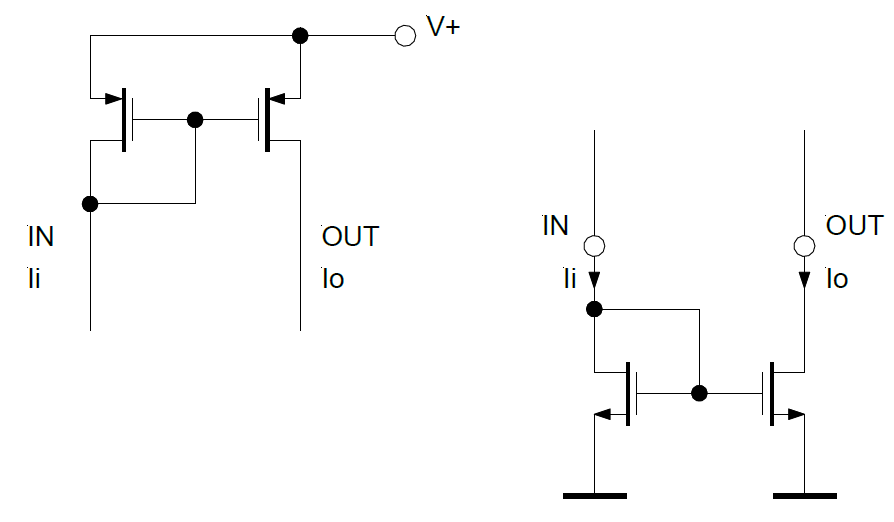
\includegraphics[width=3cm]{images/stromspiegel/widlar.png}}
		\caption{Widlar}
	\end{subfigure} \qquad	
	\begin{subfigure}[b]{3cm}
		\centering
		{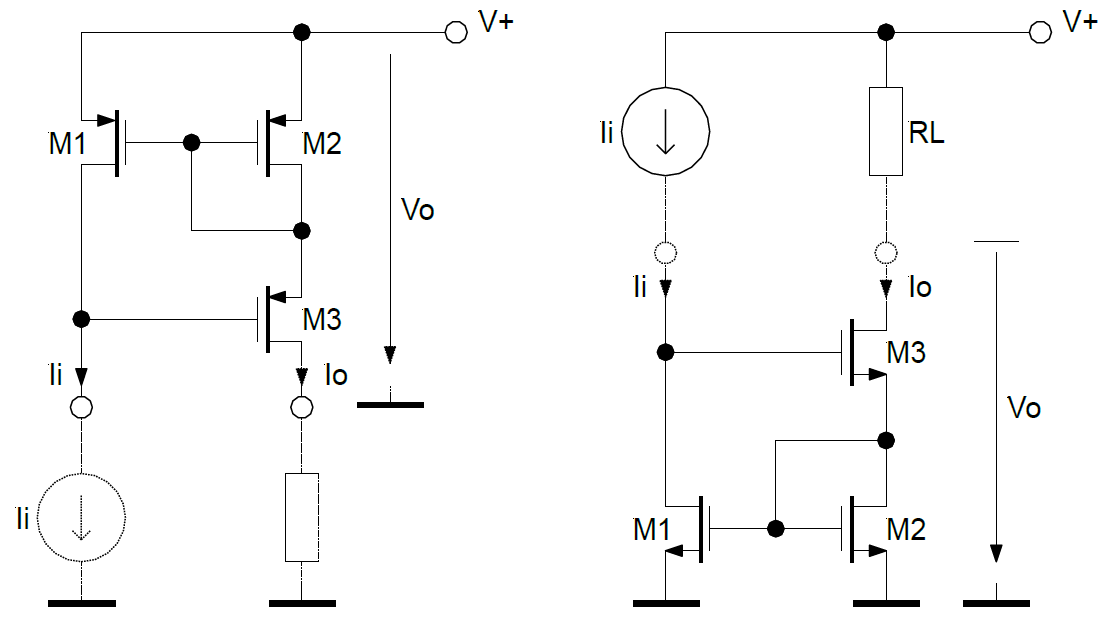
\includegraphics[width=3cm]{images/stromspiegel/wilson.png}}
		\caption{Wilson}
	\end{subfigure} \qquad	
	\begin{subfigure}[b]{3cm}
		\centering
		{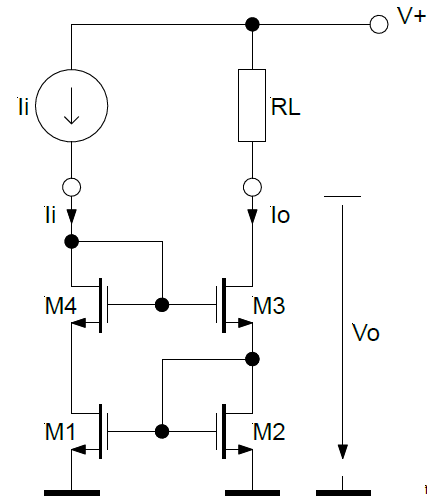
\includegraphics[width=3cm]{images/stromspiegel/verbesserter_wilson.png}}
		\caption{Verbesserter Wilson}
	\end{subfigure} \qquad	
	\begin{subfigure}[b]{3cm}
		\centering
		{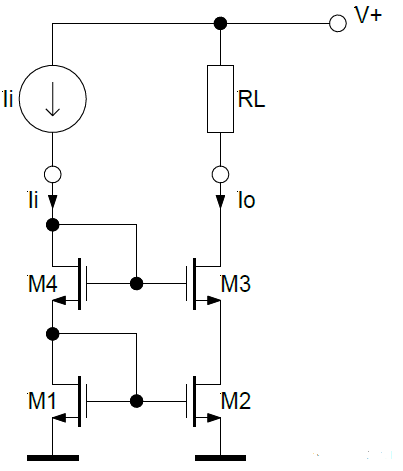
\includegraphics[width=3cm]{images/stromspiegel/kaskode.png}}
		\caption{Kaskode}
	\end{subfigure} \qquad	
	\begin{subfigure}[b]{3cm}
		\centering
		{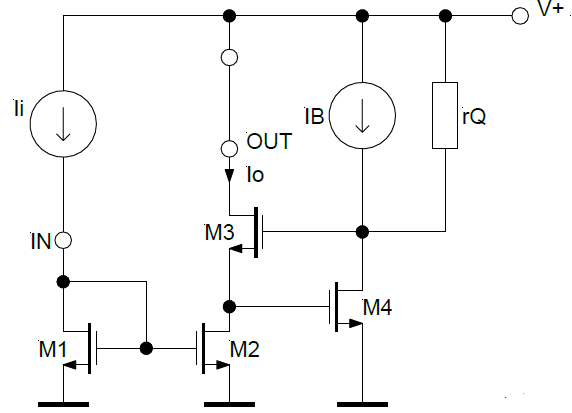
\includegraphics[width=3cm]{images/stromspiegel/geregelte_kaskode.png}}
		\caption{Geregelte Kaskode}
	\end{subfigure}
	\caption{Die Stromspiegeltypen}
	\label{fig:stromspiegeltypen}
\end{figure}

\section{Grundschaltungen mit MOS-Transistoren\skript{Kap. 6}}

\subsection{Grundschaltungen}
Die Grundschaltungen besitzen je einen Ein- und Ausgang. Derjenige Transistoranschluss, welcher weder Ein- noch Ausgang darstellt gibt der Grundschaltung
den Namen. \\

\begin{tabularx}{\linewidth}{|X|l|l|l|}
	\hline
	\textbf{Grundschaltung}	& \textbf{Eingangsanschluss} & \textbf{Ausgangsanschluss} & \textbf{Namensgebender Anschluss}
	\\ \hline
	Source Schaltung	& Gate				& Drain				& Source
	\\ \hline
	Gate Schaltung		& Source			& Drain				& Gate
	\\ \hline
	Drain Schaltung (Source-Folger) & Gate				& Source			& Drain 
	\\ \hline
\end{tabularx} \\

\textbf{Eigenschaften:} \\
\begin{tabularx}{\linewidth}{|X|l|l|}
	\hline
	\textbf{Grundschaltung} & \textbf{Typische Anwendung} & \textbf{Eingangs-/Ausgangswiderstand}
	\\ \hline
	Source Schaltung & Verstärker tiefe bis mittlere Frequenzen & gross/gross
	\\ \hline
	Gate Schaltung & Verstärker hohe Frequenzen & klein/gross
	\\ \hline
	Drain Schaltung & Spannungsfolger / Impedanzwandler & gross/klein
	\\ \hline
\end{tabularx}

\section{Einstufige MOS Verstärker\skript{Kap. 10}}

\begin{multicols}{2}

\section{Frequenzverhalten von MOS Verstärker}
Jeder Knoten N bildet einen Pol bei der Frequenz
$f_N=\frac{1}{2\pi\cdot R_NC_N}$. \\

\textbf{Grobe Analyse:} Die Knoten mit hohen RC-Produkten suchen. Dort entstehen
Systempole, welche einen Abfall von 20dB/Dekade im Frequenzgang einleiten.

\subsection{Widerstände}
	\textbf{Knotenimpedanz praktisch unendlich:} \\ Gate: $r_{iG}\rightarrow\infty$ \\
	\textbf{Knotenimpedanz sehr hoch:} \\ Drain des Transistors wenn
		als Stromquelle beschaltet: $r_{ds}=\frac{1}{g_0}$  \\	
	\textbf{Knotenimpedanz tief:} \\ Drain des Transistors in
		Diodenschaltung, Source des Transistors in Stromquellenschaltung: $\frac{1}{g_m}$  \\
		
\subsection{Kapazitäten}
	\textbf{Knotenkapazität gross:} \\ C als passive Schaltungskomponente. \\
	\textbf{Knotenkapazität mittel:} \\ parasitäre Kapazität verstärkt durch Miller-Effekt.
	Häufig $C_{GD}$ eines verstärkenden Transistors. \\
	\textbf{Knotenkapazität klein:} \\ Knoten mit parasitären Kapazitäten. In der Regel beim
	Gate-Knoten am höchsten. \\

\columnbreak

\subsection{Millerkapazität}
Die Miller Kapazität $C_M$ zwischen Ein- und Ausgang eines Verstärkers mit
Verstärker A liegt, erscheint:\\

multipliziert mit ($1-A$) parallel zum Eingang ($C_{MI}$)\\
multipliziert mit ($1-\frac{1}{A}$) parallel zum Ausgang ($C_{MO}$)\\

$C_M$ wird aus dem Schema entfernt\\

\subsection{Darstellung}
\begin{enumerate}
  \item DC Verstärkung berechnen (aus Kleinsignalersatzschaltung für
  Niederfrequenz)
  \item Die relevanten Pole finden (An welchem Knoten befindet sich ein hohes
  RC Produkt)
  \item Pole in Bode-Diagramm einzeichnen
\end{enumerate}

\subsection{Typische Kapazitäten}
\adjustbox{max width=\linewidth}{
	\begin{tabular}{|l|l|l|l|l|} 
	\hline
		& $C_{GS}$ & $C_{GD}$ & $C_{SB}$ & $C_{DB}$ \\ 
	\hline
		Gesättigt & $C_{GS0} + \frac{2}{3}C_{oxt}$ & $C_{GD0}$ & $C_{jSBt}+\frac{2}{3}C_{BCt}$ & $C_{jDBt}$ \\
 		Typ. Wert & 33 fF & 1.2 fF & 10 fF & 7 fF \\
	\hline
		Ungesättigt & $C_{GS0}+\frac{1}{2}C_{oxt}$ & $C_{GD0}+\frac{1}{2}C_{oxt}$ & $C_{jSBt}+\frac{1}{2}C_{BCt}$ & $C_{jDBt}+\frac{1}{2}C_{BCT}$ \\
		Typ. Wert & 26 fF & 26 fF & 10 fF & 10 fF \\
	\hline	
	\end{tabular}
} \\

$C_{oxt} = C_{ox} \cdot W \cdot L_{eff}  \quad C_{BCt} = C_{jBC} \cdot W \cdot L_{eff} $ \\
$C_{jSBt} = C_{jSB} \cdot A_S + C_{jswSB} \cdot P_S$ \\
$C_{jDBt} = C_{jDB} \cdot A_D + C_{jswDB} \cdot P_D$ \\

Wenn $V_{SB}=0$, dann $C_{SB}$ ignorieren und $C_{DB}=C_{DS}$.

\end{multicols}

\section{MOS Operationsverstärker}

\subsection{Struktur}
\begin{tabular}{p{3cm}p{15cm}}
	Differenzstufe (Eingangsstufe) & bildet die Differenz der Eingangssignale,
	verstärkt sie mit dem Differenz-Verstärkungsfaktor\\
	Verstärkungsstufe	(Integratorstufe) & Verstärkerstufe, erhöht die
	Gesamtverstärkung. Bestimmt meist die Gesamtbandbreite des
	Operationsverstärkers\\
	Leistungsstufe (Ausgangsstufe) & Impedanzwandler. Verstärkung ist selten
	grösser als eins. Verkleinert den Ausgangswiderstand und stellt genügend
	Ausgansstrom zur verfügung\\
\end{tabular}

\subsection{Differenzstufe}
\begin{figure}[h]
	\centering
	\begin{subfigure}[b]{5cm}
		\centering
		{\begin{circuitikz}[american, european resistors, scale=0.5, transform shape]
\ctikzset{tripoles/mos style/arrows}

\draw
	(2,2) node [nmos] (M1) {}
	(4,2) node [nmos, xscale=-1] (M2) {}
	
	(M1.S) to (M2.S)
	(M1.G) to (0.5,2) node [ocirc] {Vi1}
	(2,4.5) to [R=RD1,i=ID1] (M1.D)
	
	(M2.G) to (5.5,2) to (5.5,1) to (0.5,1) node [ocirc] {Vi2}
	(4,4.5) node [circ] {} to [R=RD2,i=ID2=Io] (M2.D)
	
	(5.5,4.5) node [ocirc] {V+} to (2,4.5)
	(3,1.25) node [circ] {} to [I] (3,-0.5) to (5.5,-0.5) node [ocirc] {V-}
;

\end{circuitikz}}
		\caption{Widerstandslast}
	\end{subfigure}\qquad
	\begin{subfigure}[b]{5cm}
		\centering
		{\begin{circuitikz}[american, european resistors, scale=0.5, transform shape]
\ctikzset{tripoles/mos style/arrows}

\draw
	(2,2) node [nmos] (M1) {}
	(4,2) node [nmos, xscale=-1] (M2) {}
	
	(M1.S) to (M2.S)
	(M1.G) to (0.5,2) node [ocirc] {Vi1}
	(2,3) to (M1.D)
	
	(M2.G) to (5.5,2) to (5.5,1) to (0.5,1) node [ocirc] {Vi2}
	(4,3) to (M2.D)
	
	(5.5,4.5) node [ocirc] {V+} to (3,4.5) to (3,4)
	(1,4) rectangle (5,3)
	(3,1.25) node [circ] {} to [I=$I_Q$] (3,-0.5) to (5.5,-0.5) node [ocirc] {V-}
	(3,3.5) node {1:1}
	(4,2.7) to [short, i<_=iout] (6,2.7) node [ocirc] {}
;

\end{circuitikz}}
		\caption{Stromspiegellast}
	\end{subfigure}
	\caption{Differenzstufen}
	\label{fig:Differenzstufen}
\end{figure}\\

\subsection{Die wichtigsten Formeln}
\begin{tabular}{p{7cm}p{11cm}}
Verstärkung Differenzstufe &
\textbf{Bei Widerstandslast} $i_{out}=-\frac{g_mv_d}{2}$
$a\approx\frac{g_m\cdot r_{out}}{2}$ \newline
\textbf{Bei Stromspiegellast} $i_{out}=-g_mv_d$ $a\approx g_m\cdot r_{out}$
\\
Grenzwert bei starker Inversion & $a=V_A\sqrt{\frac{\beta}{I_Q}}$ (Bedingung:
$a_{E_N}=a_{E_P}$)\\
Grenzwert bei schwacher Inversion & $a=\frac{V_A}{2n_M\Phi_t}$\\
Gain-Bandwith-Product & $GBP=|a|\cdot f_{P1}$ \\
Slew-Rate & $SR=\frac{dv_o}{dt}=\frac{I_{out}}{C_L}$ \\
Common mode rejection ratio & $CMRR=\left| \frac{a_{DM}}{a_{CM}}\right|$\\
Power supply rejection ratio &
$PSSR_+ = \left| \frac{a_{DM}}{a_{PS+}}\right|$ \newline
$PSSR_- = \left| \frac{a_{DM}}{a_{PS-}}\right|$ \\
Offset: Designregel & Symmetrie, gleiche Stromdichten $\frac{I}{W/L}$ in
Stromspiegeltransistoren\\
\end{tabular}


\section{Stabilität von MOS Operationsverstärker}
\begin{figure}[!h]
	\centering
	\begin{subfigure}[b]{10cm}
		\centering
		\adjustbox{scale=0.9}{\begin{tikzpicture}[scale=0.8,transform shape]
	%axis
	%x
	\foreach \x in {0,...,9} {
		\draw (\x,0) -- (\x,6.4);
		\draw (\x,6.6) -- (\x,11);
	}
	%y
	\foreach \y in {0,...,11} {
		\draw (0,\y) -- (9,\y);
	}
	\draw node at (0,-0.3) {1};
	\draw node at (1,-0.3) {10};
	\draw node at (2,-0.3) {100};
	\draw node at (3,-0.3) {1k};
	\draw node at (4,-0.3) {10k};
	\draw node at (5,-0.3) {100k};
	\draw node at (6,-0.3) {1M};
	\draw node at (7,-0.3) {10M};
	\draw node at (8,-0.3) {100M};
	\draw node at (9,-0.3) {1G};
	
	\draw node at (-0.5,0) {-300};
	\draw node at (-0.5,1) {-250};
	\draw node at (-0.5,2) {-200};
	\draw node at (-0.5,3) {-150};
	\draw node at (-0.5,4) {-100};
	\draw node at (-0.5,5) {-50};
	\draw node at (-0.5,6) {0};
	\draw node at (-0.5,7) {0};
	\draw node at (-0.5,8) {20};
	\draw node at (-0.5,9) {40};
	\draw node at (-0.5,10) {60};
	\draw node at (-0.5,11) {80};

\draw [thick, red] plot[smooth, tension=.7] coordinates {(0,6) (1.0379,5.7673) (3.0063,4.4457) (7.2804,3.7427) (8.9957,0.1716)    };
\draw [thick, green] plot[smooth, tension=.7] coordinates {(0,11) (1.6284,10.9694) (2.697,10.314) (6.0151,7.3983) (7.5335,6.5828) (9.052,6.5547)};
\draw [dashed] (6.5,11.2) -- (6.5,-0.2);
\draw [dashed] (8.3,11.2) -- (8.3,-0.2);
\draw [dashed] (-0.2,2.3) -- (9.2,2.3);
\draw [dashed] (-0.2,4.1) -- (9.2,4.1);
\draw [<->] (9.5,4.1) -- (9.5,0);
\draw node at (9.5,2) [anchor=west] {Phasenmarge};
\draw node at (6.5,11.2) [anchor=south] {$f_{krit}$};
\end{tikzpicture}
}
		\caption{Bodeplot}
	\end{subfigure}\qquad
	\begin{subfigure}[b]{8cm}
		\centering
		{\begin{tikzpicture}[scale=0.8,transform shape]
	\draw [->] (0,0) node [anchor=east] {$U_{in}$} -- (1,0);
	\draw (2,0) circle (1);
	\draw node at (2,0) {$\sum$};
	\draw [->] (3,0) -- (3.5,0);
	\draw (3.5,0.5) rectangle (5,-0.5);
	\draw node at (4.25,0) {$A(s)$};
	\draw [->] (5,0) -- (6,0) node [anchor=west] {$U_{out}$};
	\draw [->] (5.5,0) -- (5.5,2) -- (5,2);
	\draw (5,2.5) rectangle (3.5,1.5);
	\draw node at (4.25,2) {$F(s)$};
	\draw [->] (3.5,2) -- (2,2) -- (2,1);
	

\end{tikzpicture}}
		\caption{Rückgekoppelter Verstärker}
	\end{subfigure}
	\caption{Stabilität}
	\label{fig:stabilitaet}
\end{figure}

\begin{tabular}{|l|l|}
\hline
	Phasenmarge bei $f_{krit}(a_L=1)$ &
	Verhalten des Verstärkers \\
	& (System mit zwei weit auseinanderliegenden Polen) \\\hline
	$\varphi_M \leq 0^\circ$ & 
	Gegenkoppelter Verstärker schwingt selbständig \\\hline
	$\varphi_M > 0^\circ$ &
	Gedämpftes Überschwingen der Sprungantwort \\\hline
	$\varphi_M = 65^\circ$ &
	Peaking verschwindet. Einziger Überschwinger mit 4.7\% Sprunghöhe \\\hline
	$\varphi_M \geq 75^\circ$ &
	Kein Überschwingen \\\hline
\end{tabular}

\begin{tabular}{lll}
Stabilitätskriterien & $\Phi = 180^\circ$ & $ \left|A(s)\cdot F(s)\right|<1 $ \\
& $ \left|A(s)\cdot F(s)\right|= 1 $ & $ \rightarrow 180^\circ-\Phi>0;\
\varphi_M>0^\circ $ \\
Phasenmarge & $\varphi_M=180^\circ-\Phi $ & \\
Designregel & Wähle 2. Pol ($f_nd$) bei ca. $3\cdot GBP$& \\
\end{tabular}

%TODO: hässlichen newpage entfernen
\newpage

\section{Gebräuchliche Realisierung von OTA's}
Ein einstufiger OTA wird bereits durch die Differenzstufe realisiert. Dies ist jedoch nicht praktisch da die Last am
Ausgang die Symmetrie der Differenzstufe stört.
Schaltungen siehe Abbildung \ref{fig:otas}!
\begin{figure}[htp]
\begin{center}
	\begin{subfigure}[b]{0.49\linewidth}
		\centering
		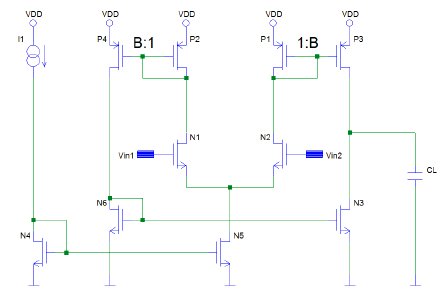
\includegraphics[width=0.9\linewidth]{images/SymetrischerOTA.png}
		\caption{Symmetrischer OTA}
	\end{subfigure}
	\begin{subfigure}[b]{0.49\linewidth}
		\centering
		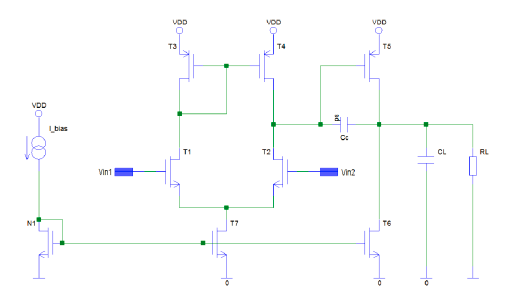
\includegraphics[width=0.9\linewidth]{images/millerOTA.png}
		\caption{Miller OTA}
	\end{subfigure}
	\caption{Gebräuchliche Realisierungen von OTA's}
	\label{fig:otas}
\end{center}
\end{figure}

\textbf{Verstärkungen:} \\
\begin{tabular}{lll}
	Symmetrischer OTA:	& & $a_v = B \cdot g_{m_{N1}} \cdot (r_{DS_{N3}} || r_{DS_{P3}})$ \\
	Miller OTA:			& & $a_v = a_{v1} \cdot a_{v2} = g_{m1}(r_{DS2} || r_{DS4}) \cdot g_{m5}(r_{DS5} || r_{DS6} || R_L)$
\end{tabular}

\subsection{Designgleichungen Miller OTA}
\begin{tabular}{|l|l|} \hline
	Verstärkung & $a = A_1 \cdot A_2 = g_{m1} \cdot R_{N2} \cdot g_{m5} \cdot R_{N3}$ \\ \hline
	Dominanter Pol & $f_{pN2} = \frac{1}{2\pi R_{N2} (C_{N2}+A_2C_c)} \approx \frac{1}{2\pi R_{N2}A_2C_c}$ \\ \hline
	3dB-Bandwidth & $BW \approx f_d = f_{N2} = \frac{1}{2\pi \cdot R_{N2} \cdot A_2C_c}$ \\ \hline
	Gain-Bandwith & $GBP = a \cdot f_d = \frac{g_{m1} \cdot R_{N2} \cdot g_{m5} \cdot R_{N3}}{2\pi \cdot R_{N2} \cdot A_2C_c} = \frac{g_{m1}}{2\pi C_c}$ \\ \hline
	Nondominanter Pol & $f_{nd} = f_{N3} = \frac{1}{2\pi \cdot R_{N3} \cdot C_L} \approx \frac{g_{m5}}{2\pi C_L}$ \\ \hline
	Phasenmarge & $\phi_m = 90^\circ - \arctan \frac{GBW}{f_{nd}}$ \\ \hline
	Nullstelle & $f_z \approx \frac{g_{m5}}{2\pi C_c}$ \\ \hline
\end{tabular}

%\section{Designprojekt OTA}
Vorgaben:
\begin{description}[noitemsep, leftmargin=4.2cm, style=sameline]
  \item[Open-Loop-Gain:] $\geq 80 dB$
  \item[Last:] $\leq 5 pF$
  \item[GBW:] $\geq 5 MHz$
  \item[Phase Margin:] $\geq 60^\circ$
  \item[Stabilität:] Unity-Gain stable
  \item[Slew-Rate:] $\geq 20V/\mu S$
  \item[Versorgungsspannung:] $3.3V$
  \item[Output-Swing:] (VSS + 500mV) \ldots (VDD-500mV)
\end{description}

\subsection{Design Ablauf}
OTA wird typischerweise ein Sub-Block einer grösseren Schaltung sein.

\begin{enumerate}[noitemsep]
  \item Definition der Ein- und Ausgägne einer Schaltung (Spezifikation der Schaltung)
  \item Handberechnung, Erstellung des Schaltplanes
  \item Schaltkreissimulation
  \item Erfüllt der Schaltkreis die Spezifikation? Wenn nein, zurück zu 1. Sonst weiter.
  \item Layout
  \item Schaltkreissimulation mit parasitären Einflüssen
  \item Erfüllt der Schaltkreis die Spezifikationen? Nein: Zurück zu Layout, sonst weiter.
  \item Herstellung eines Prototypen
  \item Test und Evaluation
  \item Erfüllt der Schaltkreis die Spezifikation? Nein: Zurück zur Herstellung Prototyp oder zurück zu 1.
  \item Produktion
\end{enumerate}

\section{Spannungsreferenzen}
\begin{figure}[!h]
	\centering
	\begin{subfigure}[b]{10cm}
		\centering
	%	{\begin{tikzpicture}[scale=0.8,transform shape]
	%axis
	%x
	\foreach \x in {0,...,9} {
		\draw (\x,0) -- (\x,6.4);
		\draw (\x,6.6) -- (\x,11);
	}
	%y
	\foreach \y in {0,...,11} {
		\draw (0,\y) -- (9,\y);
	}
	\draw node at (0,-0.3) {1};
	\draw node at (1,-0.3) {10};
	\draw node at (2,-0.3) {100};
	\draw node at (3,-0.3) {1k};
	\draw node at (4,-0.3) {10k};
	\draw node at (5,-0.3) {100k};
	\draw node at (6,-0.3) {1M};
	\draw node at (7,-0.3) {10M};
	\draw node at (8,-0.3) {100M};
	\draw node at (9,-0.3) {1G};
	
	\draw node at (-0.5,0) {-300};
	\draw node at (-0.5,1) {-250};
	\draw node at (-0.5,2) {-200};
	\draw node at (-0.5,3) {-150};
	\draw node at (-0.5,4) {-100};
	\draw node at (-0.5,5) {-50};
	\draw node at (-0.5,6) {0};
	\draw node at (-0.5,7) {0};
	\draw node at (-0.5,8) {20};
	\draw node at (-0.5,9) {40};
	\draw node at (-0.5,10) {60};
	\draw node at (-0.5,11) {80};

\draw [thick, red] plot[smooth, tension=.7] coordinates {(0,6) (1.0379,5.7673) (3.0063,4.4457) (7.2804,3.7427) (8.9957,0.1716)    };
\draw [thick, green] plot[smooth, tension=.7] coordinates {(0,11) (1.6284,10.9694) (2.697,10.314) (6.0151,7.3983) (7.5335,6.5828) (9.052,6.5547)};
\draw [dashed] (6.5,11.2) -- (6.5,-0.2);
\draw [dashed] (8.3,11.2) -- (8.3,-0.2);
\draw [dashed] (-0.2,2.3) -- (9.2,2.3);
\draw [dashed] (-0.2,4.1) -- (9.2,4.1);
\draw [<->] (9.5,4.1) -- (9.5,0);
\draw node at (9.5,2) [anchor=west] {Phasenmarge};
\draw node at (6.5,11.2) [anchor=south] {$f_{krit}$};
\end{tikzpicture}
}
		\caption{Prinzip der Spannungsreferenz}
	\end{subfigure}\qquad
	\begin{subfigure}[b]{8cm}
		\centering
		%{\begin{tikzpicture}[scale=0.8,transform shape]
	\draw [->] (0,0) node [anchor=east] {$U_{in}$} -- (1,0);
	\draw (2,0) circle (1);
	\draw node at (2,0) {$\sum$};
	\draw [->] (3,0) -- (3.5,0);
	\draw (3.5,0.5) rectangle (5,-0.5);
	\draw node at (4.25,0) {$A(s)$};
	\draw [->] (5,0) -- (6,0) node [anchor=west] {$U_{out}$};
	\draw [->] (5.5,0) -- (5.5,2) -- (5,2);
	\draw (5,2.5) rectangle (3.5,1.5);
	\draw node at (4.25,2) {$F(s)$};
	\draw [->] (3.5,2) -- (2,2) -- (2,1);
	

\end{tikzpicture}}
		%TODO
		\caption{Praktische Schaltung}
	\end{subfigure}
	\caption{Bandgap-Schaltungen}
	\label{fig:spannungsreferenzen}
\end{figure}

$V_{ref}=V_D+K\cdot \Phi_t$\\
$\Phi_t = \frac{kT}{e}$, ist bei Raumtemperatur $27^\circ C$ $\Phi_t=25.9mV$\\
\begin{tabular}{ll}
Boltzmann-Konstante & $k=1.38\cdot 10^{-23}\frac{J}{K}$\\
absolute Temperatur & T = Temperatur in Kelvin\\
Elementarladung & $e=1.60\cdot 10^{-19}C$\\
\end{tabular}\\
\textbf{Realisierung:}\\
Die beiden Emitterflächen werden mit $A_1$ bzw. $A_2$ bezeichnet.\\
$V_{ref}=V_{EB1}+\Phi_t\cdot\frac{R_2}{R_3}\cdot\ln\left(\frac{R_2}{R_1}\cdot\frac{A_2}{A_1}\right)$

\appendix

\section{Technologieparameter}

\begin{tabularx}{\linewidth}{|X|l|ll|}
	\hline
		\textbf{Parameter} & \textbf{N-Kanal Transistor} & \textbf{P-Kanal Transistor} &
	\\ \hline
		$V_T$ & $0.65V \: (\pm 0.15V)$ & $0.8V \: (\pm 0.15V)$ &
	\\ \hline
		$\beta_0$ & $80 \mu A / V^2$ & $30 \mu A / V^2$ &
	\\ \hline
		$\lambda$ (Body Effekt Konstante) & $0.6V^{1/2}$ & $0.5 V^{1/2}$ & 
	\\ \hline
		\multirow{2}{*}{$a_A$ (Early-Faktor)} & $17V/\mu m$ in strong inversion & $15V/\mu m$ in strong inversion &
	\\
		& $10V/\mu m$ in weak inversion & $8.8V/\mu m$ in weak inversion &
	\\ \hline
		$n_M$ (subtreshold slope factor) & 1.5 & 1.5 &
	\\ \hline
		$I_M'$ & $20nA$ & $-10nA$ &
	\\ \hline
		$I_H'$ & $700nA$ & $-300nA$ &
	\\ \hline
		$V_M-V_T$ & $-60mV$ & $60mV$ &
	\\ \hline
		$V_H-V_T$ & $160mV$ & $-160mV$ &
	\\ \hline
		Poly-Widerstand & \multicolumn{2}{c}{$33 \Omega / \diamond$} &
	\\ \hline
		Metall-Poly Kapazität (IN1-PS) & \multicolumn{2}{c}{$0.056 fF / \mu m^2$} &
	\\ \hline
\end{tabularx}
\end{document}
